\documentclass[tikz,border=5mm]{standalone}
\usepackage[T1]{fontenc}
\usepackage{lmodern}
\usetikzlibrary{arrows.meta}
\renewcommand{\familydefault}{\sfdefault}
\begin{document}
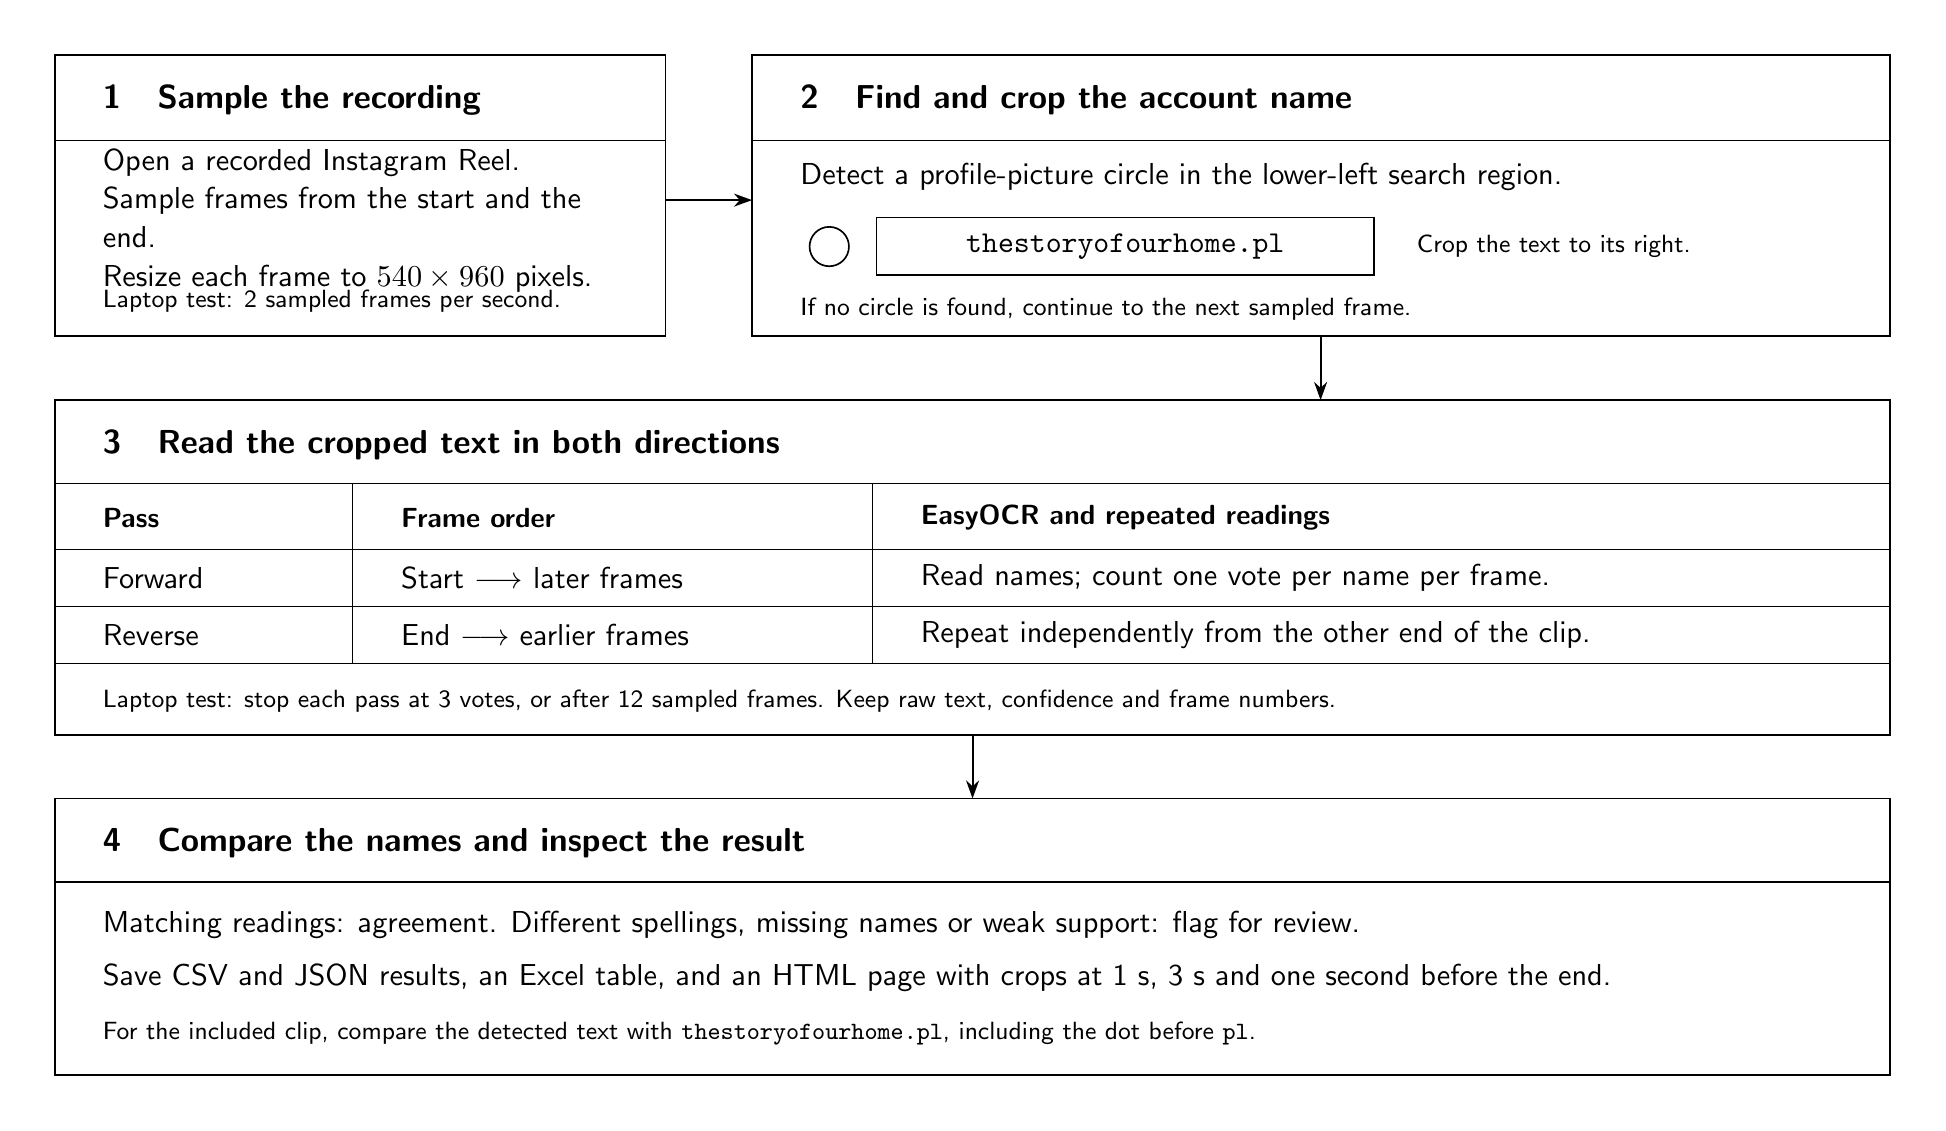
\begin{tikzpicture}[x=1cm,y=1cm,font=\sffamily,text=black,
  box/.style={draw=black,fill=white,line width=.6pt},
  flow/.style={-{Stealth[length=2.3mm,width=1.65mm]},line width=.75pt},
  heading/.style={font=\bfseries\fontsize{12}{15}\selectfont,align=left},
  body/.style={font=\fontsize{10.5}{14}\selectfont,align=left},
  small/.style={font=\fontsize{9.5}{12.5}\selectfont,align=left},
  column/.style={font=\bfseries\fontsize{10}{13}\selectfont,align=left}]
\useasboundingbox (0,0) rectangle (24,13.65);
\fill[white] (0,0) rectangle (24,13.65);

% RECORDING AND CROP
\draw[box] (.35,9.73) rectangle (8.10,13.3);
\node[heading,anchor=west] at (.83,12.73) {1\quad Sample the recording};
\draw[line width=.4pt] (.35,12.22)--(8.10,12.22);
\node[body,anchor=west,text width=6.6cm] at (.83,11.2)
  {Open a recorded Instagram Reel.\\Sample frames from the start and the end.\\Resize each frame to $540\times960$ pixels.};
\node[small,anchor=west] at (.83,10.18) {Laptop test: 2 sampled frames per second.};

\draw[box] (9.20,9.73) rectangle (23.65,13.3);
\node[heading,anchor=west] at (9.69,12.73) {2\quad Find and crop the account name};
\draw[line width=.4pt] (9.20,12.22)--(23.65,12.22);
\node[body,anchor=west] at (9.69,11.76)
  {Detect a profile-picture circle in the lower-left search region.};
\draw[line width=.6pt] (10.18,10.87) circle (.25);
\draw[box] (10.78,10.51) rectangle (17.1,11.24);
\node[body,anchor=center] at (13.94,10.875) {\texttt{thestoryofourhome.pl}};
\node[small,anchor=west] at (17.52,10.875) {Crop the text to its right.};
\node[small,anchor=west] at (9.69,10.08) {If no circle is found, continue to the next sampled frame.};
\draw[flow] (8.10,11.46)--(9.20,11.46);
\draw[flow] (16.42,9.73)--(16.42,8.92);

% TWO PASSES SHARE ONE OCR METHOD
\draw[box] (.35,4.67) rectangle (23.65,8.92);
\node[heading,anchor=west] at (.83,8.35) {3\quad Read the cropped text in both directions};
\draw[line width=.4pt] (.35,7.86)--(23.65,7.86);
\node[column,anchor=west] at (.83,7.43) {Pass};
\node[column,anchor=west] at (4.62,7.43) {Frame order};
\node[column,anchor=west] at (11.22,7.43) {EasyOCR and repeated readings};
\draw[line width=.4pt] (.35,7.02)--(23.65,7.02);
\draw[line width=.4pt] (4.13,5.57)--(4.13,7.86);
\draw[line width=.4pt] (10.73,5.57)--(10.73,7.86);
\node[body,anchor=west] at (.83,6.66) {Forward};
\node[body,anchor=west] at (4.62,6.66) {Start $\longrightarrow$ later frames};
\node[body,anchor=west] at (11.22,6.66) {Read names; count one vote per name per frame.};
\draw[line width=.35pt] (.35,6.3)--(23.65,6.3);
\node[body,anchor=west] at (.83,5.94) {Reverse};
\node[body,anchor=west] at (4.62,5.94) {End $\longrightarrow$ earlier frames};
\node[body,anchor=west] at (11.22,5.94) {Repeat independently from the other end of the clip.};
\draw[line width=.4pt] (.35,5.57)--(23.65,5.57);
\node[small,anchor=west] at (.83,5.1)
  {Laptop test: stop each pass at 3 votes, or after 12 sampled frames. Keep raw text, confidence and frame numbers.};
\draw[flow] (12,4.67)--(12,3.86);

% COMPARISON AND REVIEW
\draw[box] (.35,.35) rectangle (23.65,3.86);
\node[heading,anchor=west] at (.83,3.29) {4\quad Compare the names and inspect the result};
\draw[line width=.4pt] (.35,2.80)--(23.65,2.80);
\node[body,anchor=west] at (.83,2.26)
  {Matching readings: agreement. Different spellings, missing names or weak support: flag for review.};
\node[body,anchor=west] at (.83,1.58)
  {Save CSV and JSON results, an Excel table, and an HTML page with crops at 1 s, 3 s and one second before the end.};
\node[small,anchor=west] at (.83,.88)
  {For the included clip, compare the detected text with \texttt{thestoryofourhome.pl}, including the dot before \texttt{pl}.};
\end{tikzpicture}
\end{document}
